% Tema acadêmico UEFS para Beamer (PDF). Par do academico.css/academico.html.
% Os textos institucionais e as faixas da régua são definidos pelo filtro
% academico.lua a partir do YAML de cada apresentação.

\usetheme{default}
\usefonttheme{professionalfonts}
\usepackage{tikz}
\usetikzlibrary{arrows.meta}

\definecolor{academicoazul}{HTML}{1F4268}
\definecolor{academicoazulescuro}{HTML}{16324F}
\definecolor{academicoouro}{HTML}{B38A3D}
\definecolor{academicocinza}{HTML}{5B6573}
\definecolor{academicofundo}{HTML}{F7F9FC}
\definecolor{academicotexto}{HTML}{26313D}

\setbeamercolor{normal text}{fg=academicotexto,bg=white}
\setbeamercolor{structure}{fg=academicoazul}
\setbeamercolor{alerted text}{fg=academicoazulescuro}
\setbeamercolor{frametitle}{fg=academicoazulescuro,bg=white}
\setbeamercolor{framesubtitle}{fg=academicocinza}
\setbeamercolor{section title}{fg=academicoazulescuro}
\setbeamercolor{section page}{fg=academicoazulescuro,bg=academicofundo}
\setbeamercolor{block title}{fg=white,bg=academicoazul}
\setbeamercolor{block body}{fg=academicotexto,bg=academicoazul!5}
\setbeamercolor{block title alerted}{fg=white,bg=academicoouro!90!black}
\setbeamercolor{block body alerted}{fg=academicotexto,bg=academicoouro!10}
\setbeamercolor{block title example}{fg=academicoazulescuro,bg=academicoazul!15}
\setbeamercolor{block body example}{fg=academicotexto,bg=academicoazul!5}
\setbeamercolor{caption name}{fg=academicocinza}
\setbeamercolor{caption}{fg=academicocinza}

\setbeamerfont{title}{size=\LARGE,series=\bfseries}
\setbeamerfont{subtitle}{size=\large}
\setbeamerfont{author}{size=\normalsize}
\setbeamerfont{institute}{size=\small}
\setbeamerfont{date}{size=\small}
\setbeamerfont{frametitle}{size=\large,series=\bfseries}
\setbeamerfont{section title}{size=\LARGE,series=\bfseries}
\setbeamerfont{block title}{series=\bfseries}
\setbeamerfont{caption}{size=\scriptsize}
\setbeamertemplate{caption}{\raggedright\insertcaption\par}

% Textos padrão; o filtro sobrescreve com os valores do YAML.
\providecommand{\AcademicHeaderOne}{UNIVERSIDADE ESTADUAL DE FEIRA DE SANTANA}
\providecommand{\AcademicHeaderTwo}{}
\providecommand{\AcademicHeaderThree}{}
\providecommand{\AcademicFooterLabel}{UEFS}
\providecommand{\AcademicSecondLine}{}
\providecommand{\AcademicPlaceLine}{Feira de Santana -- Bahia}
\providecommand{\AcademicRibbon}{fundo.png}
\providecommand{\AcademicSectionCount}{1}
\providecommand{\AcademicExpectedTotal}{1}
\providecommand{\AcademicIntroFrames}{1}
\providecommand{\AcademicSectionRanges}{}

% Marcador numérico redondo ([1]{.circle}).
\newcommand{\AcademicCircle}[1]{%
  \tikz[baseline=(academiccircle.base)]\node[circle,fill=academicoazul,text=white,
    inner sep=0pt,minimum size=1.45em,font=\scriptsize\bfseries] (academiccircle) {#1};}

\setbeamertemplate{navigation symbols}{}
\setbeamertemplate{blocks}[rounded][shadow=false]
\setbeamertemplate{frametitle}{%
  \nointerlineskip%
  \begin{beamercolorbox}[wd=\paperwidth,sep=0pt,leftskip=0.72cm,rightskip=0.72cm]{frametitle}%
    \vbox{}\vskip0.22cm%
    \usebeamerfont{frametitle}\strut\insertframetitle\strut\par%
    \vskip0.08cm%
    {\color{academicoouro}\rule{0.95cm}{1.3pt}}%
    \par\vskip0.08cm%
  \end{beamercolorbox}%
}

% Régua de progresso: cada traço é um slide; as larguras das seções são
% proporcionais ao número de slides. Opacidade de 55% na régua e legendas.
\newcommand{\AcademicRulerOpacity}{0.55}
\newcommand{\AcademicSegment}[4]{%
  \pgfmathsetmacro{\segleft}{(#2-1)/\AcademicTotal*\AcademicWidth}%
  \pgfmathsetmacro{\segright}{#3/\AcademicTotal*\AcademicWidth}%
  \pgfmathsetmacro{\segdone}{min(#3,max(#2-1,\AcademicCurrent))/\AcademicTotal*\AcademicWidth}%
  \def\AcademicSegmentColor{academicoazul}%
  \ifnum\value{section}=#1\relax
    \def\AcademicSegmentColor{academicoouro}%
  \fi
  \fill[academicoazul!10] (\segleft+0.7,8) rectangle (\segright-0.7,12);
  \ifnum\AcademicCurrent<#2\relax\else
    \fill[\AcademicSegmentColor] (\segleft+0.7,8) rectangle (\segdone-0.7,12);
  \fi
  \draw[academicocinza!55,line width=0.35pt] (\segleft,6) -- (\segleft,13);
  \ifnum\value{section}=#1\relax
    \node[font=\fontsize{5.4}{6}\selectfont\bfseries,text=academicoazulescuro]
      at ({(\segleft+\segright)/2},0) {#4};
  \else
    \node[font=\fontsize{5.4}{6}\selectfont,text=academicocinza]
      at ({(\segleft+\segright)/2},0) {#4};
  \fi
}
\setbeamertemplate{footline}{%
  \def\AcademicFootLeft{0.72cm}%
  \ifnum\value{framenumber}=1\relax\def\AcademicFootLeft{1.90cm}\fi%
  \leavevmode\hbox{\hspace*{\AcademicFootLeft}%
    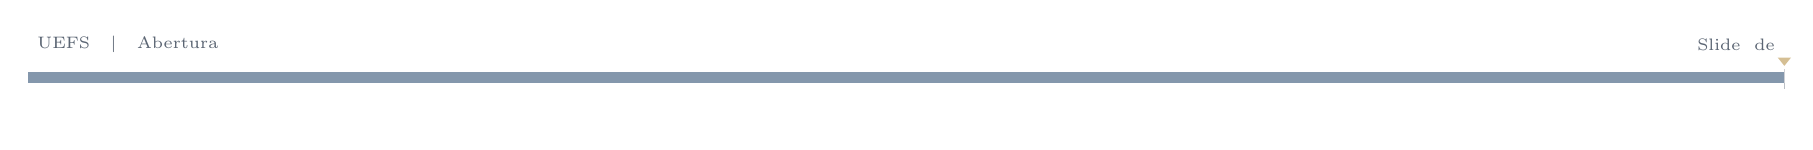
\begin{tikzpicture}[x=1pt,y=1pt]
      \pgfmathsetmacro{\AcademicWidth}{\paperwidth-\AcademicFootLeft-0.72cm}%
      \pgfmathtruncatemacro{\AcademicTotal}{max(\AcademicExpectedTotal,\inserttotalframenumber)}%
      \pgfmathtruncatemacro{\AcademicCurrent}{min(\AcademicTotal,\insertframenumber)}%
      \path[use as bounding box] (0,-6) rectangle (\AcademicWidth,28);
      \node[anchor=west,font=\fontsize{5.7}{7}\selectfont,text=academicocinza]
        at (0,22) {\AcademicFooterLabel\quad\textbar\quad
          \ifnum\value{section}=0\relax Abertura\else Etapa \insertsectionnumber/\AcademicSectionCount\fi};
      \node[anchor=east,font=\fontsize{6.5}{8}\selectfont,text=academicocinza]
        at (\AcademicWidth,22) {Slide \insertframenumber{} de \inserttotalframenumber};
      \begin{scope}[opacity=\AcademicRulerOpacity]
      \pgfmathsetmacro{\AcademicPosition}{\AcademicCurrent/\AcademicTotal*\AcademicWidth}%
      % A abertura (capa e slides anteriores à primeira seção) ocupa o primeiro intervalo.
      \pgfmathsetmacro{\AcademicIntroEnd}{min(\AcademicIntroFrames,\AcademicCurrent)/\AcademicTotal*\AcademicWidth}%
      \fill[academicoazul] (0,8) rectangle (\AcademicIntroEnd,12);
      \AcademicSectionRanges
      \foreach \step in {1,...,\AcademicTotal}{%
        \pgfmathsetmacro{\tickx}{\step/\AcademicTotal*\AcademicWidth}%
        \draw[academicocinza!45,line width=0.2pt] (\tickx,6) -- (\tickx,8);
      }
      \fill[academicoouro] (\AcademicPosition,14.2) -- ++(-2.4,3) -- ++(4.8,0) -- cycle;
      \draw[academicocinza!55,line width=0.35pt] (\AcademicWidth,6) -- (\AcademicWidth,13);
      \end{scope}
    \end{tikzpicture}%
  }%
}

\setbeamertemplate{title page}{%
  \begin{tikzpicture}[remember picture,overlay]
    \node[anchor=north west,inner sep=0pt]
      at (current page.north west)
      {\includegraphics[height=\paperheight]{\AcademicRibbon}};
    \node[anchor=north,inner sep=0pt,text width=12.6cm,align=center,
      font=\fontsize{9.5}{12}\selectfont,text=academicoazulescuro]
      at ([xshift=8.65cm,yshift=-0.72cm]current page.north west)
      {\textbf{\AcademicHeaderOne}\\[4pt]
       \AcademicHeaderTwo\\[3pt]
       \AcademicHeaderThree};
    \draw[academicoazul!20,line width=0.5pt]
      ([xshift=1.90cm,yshift=-2.20cm]current page.north west) -- ++(13.32cm,0);
    % Título e subtítulo num único bloco centrado entre o filete e o autor.
    \node[anchor=center,inner sep=0pt,text width=13cm,align=center]
      at ([xshift=0.65cm,yshift=-3.78cm]current page.north)
      {\hyphenpenalty=10000\exhyphenpenalty=10000
       {\fontsize{16}{19.5}\selectfont\bfseries\color{academicoazulescuro}\inserttitle\par}
       \vskip7pt
       {\fontsize{11.5}{14.5}\selectfont\color{academicocinza}\insertsubtitle\par}};
    \node[anchor=north,inner sep=0pt,text width=13.5cm,align=center,
      font=\fontsize{11}{14}\selectfont,text=academicotexto]
      at ([xshift=0.65cm,yshift=-5.65cm]current page.north) {\textbf{\insertauthor}};
    \node[anchor=north,inner sep=0pt,text width=13.5cm,align=center,
      font=\fontsize{9.5}{12}\selectfont,text=academicocinza]
      at ([xshift=0.65cm,yshift=-6.25cm]current page.north) {\AcademicSecondLine};
    \node[anchor=north,inner sep=0pt,font=\fontsize{8}{10}\selectfont,text=academicocinza]
      at ([xshift=0.65cm,yshift=-7.25cm]current page.north) {\AcademicPlaceLine};
  \end{tikzpicture}%
}

\setbeamertemplate{section page}{%
  \begin{tikzpicture}[remember picture,overlay]
    \node[anchor=north west,inner sep=0pt,font=\fontsize{9}{11}\selectfont,text=academicocinza]
      at ([xshift=0.85cm,yshift=-2.70cm]current page.north west)
      {ETAPA \insertsectionnumber{} DE \AcademicSectionCount};
    \node[anchor=north west,inner sep=0pt,text width=14cm,align=left,
      font=\fontsize{24}{29}\selectfont\bfseries,text=academicoazulescuro]
      at ([xshift=0.85cm,yshift=-3.35cm]current page.north west) {\insertsection};
    \draw[academicoouro,line width=2pt]
      ([xshift=0.85cm,yshift=-4.90cm]current page.north west) -- ++(1.40cm,0);
  \end{tikzpicture}%
}

\AtBeginSection{%
  \begingroup
  \setbeamercolor{background canvas}{bg=academicofundo}%
  \frame{\sectionpage}%
  \endgroup
}

% Leitura confortável em tabelas, listas e blocos densos.
\setlength{\tabcolsep}{4pt}
\renewcommand{\arraystretch}{1.06}
\setlength{\parskip}{2pt plus 1pt minus 1pt}
\setlength{\topsep}{2pt plus 1pt minus 1pt}
\setlength{\partopsep}{0pt}
\setlength{\itemsep}{1pt plus 1pt minus 1pt}
\setbeamertemplate{itemize item}{\color{academicoouro}\small\raisebox{0.15ex}{\textbullet}}
\setbeamertemplate{itemize subitem}{\color{academicoazul}\scriptsize\raisebox{0.15ex}{\textbullet}}
\setbeamertemplate{enumerate item}{\color{academicoazul}\insertenumlabel.}

\AtBeginEnvironment{longtable}{\fontsize{8.4}{10.2}\selectfont\setlength{\tabcolsep}{3pt}\setlength{\LTpre}{2pt}\setlength{\LTpost}{3pt}\renewcommand{\arraystretch}{1.04}}
\AtBeginEnvironment{tabular}{\setlength{\tabcolsep}{4pt}\renewcommand{\arraystretch}{1.10}}
\AtBeginEnvironment{verbatim}{\scriptsize}
\setbeamersize{text margin left=0.72cm,text margin right=0.72cm}
\setbeamerfont{block body}{size=\small}
\setbeamerfont{block body alerted}{size=\small}
\setbeamerfont{block body example}{size=\small}

\hypersetup{colorlinks=true,linkcolor=academicoazul,urlcolor=academicoazul}
